% Drawing 70/01-2 -- folder 70, batch 01, archive page 15 (PDF page 16).
% Transcription: matrice par blocs de $\sigma_i$, $(n+2)\times(n+2)$ : bloc identité d'ordre $i-1$ en haut à gauche ; bloc $2\times 2$ $\begin{pmatrix}0&1\\1&0\end{pmatrix}$ aux places $i,i+1$ ; à droite, sur les lignes $1$ à $i+1$, les coefficients $\lambda_{i1}\ \lambda_{i1}\cdots\lambda_{i1}$, \ldots, $\lambda_{ii}\cdots\lambda_{ii}$, $\lambda_{i,i+1}\cdots\lambda_{i,i+1}$ ; sur les $n-i$ dernières lignes, la diagonale $\lambda_{i,i+2}$ ; dernière colonne de translation nulle, $1$ en bas à droite. Les accolades marquent « $i-1$ », « $2$ », « $n-i$ », « $i+1$ ».
% Kind: block matrix of sigma_i (written out). Method 2 (schematic redraw from the facsimile). Status: partial.
% Notes: The matrix of sigma_i written as an array: identity block of order i-1 (1, dots, 1), the block (0 1 / 1 0) at places i, i+1, a large 0 below it; to the right the rows lambda_{i1} ... lambda_{i1}, ..., lambda_{ii} ... (overinked), lambda_{i,i+1} ..., then the diagonal lambda_{i,i+2}; last column 0 ... 0, 1 at the bottom right; braces i-1, 2, n-i on the left and i+1, n-i on the right. Entries are placed as text in their positions; the overinked row is given as the transcription reads it.
% Coordinates: 1 unit = 1 mm = 1/100 of the crop width (bbox in page fractions: [0.12, 0.64, 0.92, 0.84]).
% Redrawn by Claude (claude-opus-5-5), issue #73, 2026-11-07; not checked by a human; not compiled (no TeX in the session).
% Rights: reproduces part of the work -- behind RENDER_TRANSCRIPTS, never published by itself.
\documentclass[tikz,border=3pt]{standalone}
\usepackage{amsmath,amssymb}
\usetikzlibrary{patterns,arrows.meta}
\tikzset{pencil/.style={black!45}, struck/.style={black!35}, mark/.style={circle,draw,inner sep=1.3pt}, pt/.style={circle,fill,inner sep=0.9pt}, opt/.style={circle,draw,fill=white,inner sep=1.1pt}}
\begin{document}
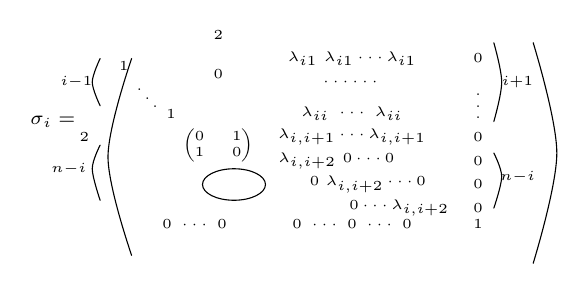
\begin{tikzpicture}[x=1mm,y=1mm,line cap=round,line join=round,font=\scriptsize]
\draw plot[smooth, tension=0.55] coordinates {(40,-6) (37,-18.5) (40,-31)};
\draw plot[smooth, tension=0.55] coordinates {(91,-4) (94,-18) (91,-32)};
\node[inner sep=1pt] at (30,-14) {\scriptsize $\sigma_i=$};
\node[inner sep=1pt] at (39,-7) {\tiny $1$};
\node[inner sep=1pt] at (42,-10) {\tiny $\ddots$};
\node[inner sep=1pt] at (45,-13) {\tiny $1$};
\node[inner sep=1pt] at (51,-3) {\tiny $2$};
\node[inner sep=1pt] at (51,-8) {\tiny $0$};
\node[inner sep=1pt] at (51,-17) {\tiny $\begin{pmatrix}0&1\\1&0\end{pmatrix}$};
\draw (53,-22) ellipse[x radius=4, y radius=2];
\node[inner sep=1pt] at (48,-27) {\tiny $0\ \cdots\ 0$};
\node[inner sep=1pt] at (68,-27) {\tiny $0\ \cdots\ 0\ \cdots\ 0$};
\node[inner sep=1pt] at (84,-27) {\tiny $1$};
\node[inner sep=1pt] at (68,-6) {\tiny $\lambda_{i1}\ \lambda_{i1}\cdots\lambda_{i1}$};
\node[inner sep=1pt] at (68,-9) {\tiny $\cdots\cdots$};
\node[inner sep=1pt] at (68,-13) {\tiny $\lambda_{ii}\ \cdots\ \lambda_{ii}$};
\node[inner sep=1pt] at (68,-16) {\tiny $\lambda_{i,i+1}\cdots\lambda_{i,i+1}$};
\node[inner sep=1pt] at (66,-19) {\tiny $\lambda_{i,i+2}\ 0\cdots 0$};
\node[inner sep=1pt] at (70,-22) {\tiny $0\ \lambda_{i,i+2}\cdots 0$};
\node[inner sep=1pt] at (74,-25) {\tiny $0\cdots\lambda_{i,i+2}$};
\node[inner sep=1pt] at (84,-6) {\tiny $0$};
\node[inner sep=1pt] at (84,-16) {\tiny $0$};
\node[inner sep=1pt] at (84,-19) {\tiny $0$};
\node[inner sep=1pt] at (84,-22) {\tiny $0$};
\node[inner sep=1pt] at (84,-25) {\tiny $0$};
\node[inner sep=1pt] at (84,-11) {\tiny $\vdots$};
\draw plot[smooth, tension=0.55] coordinates {(36,-6) (35,-9) (36,-12)};
\node[inner sep=1pt] at (33,-9) {\tiny $i{-}1$};
\node[inner sep=1pt] at (34,-16) {\tiny $2$};
\draw plot[smooth, tension=0.55] coordinates {(36,-17) (35,-20) (36,-24)};
\node[inner sep=1pt] at (32,-20) {\tiny $n{-}i$};
\draw plot[smooth, tension=0.55] coordinates {(86,-4) (87,-9) (86,-14)};
\node[inner sep=1pt] at (89,-9) {\tiny $i{+}1$};
\draw plot[smooth, tension=0.55] coordinates {(86,-18) (87,-21) (86,-25)};
\node[inner sep=1pt] at (89,-21) {\tiny $n{-}i$};
\end{tikzpicture}
\end{document}
